\begin{figure}[htbp]
			\centering
			\resizebox{\textwidth}{!}{%
				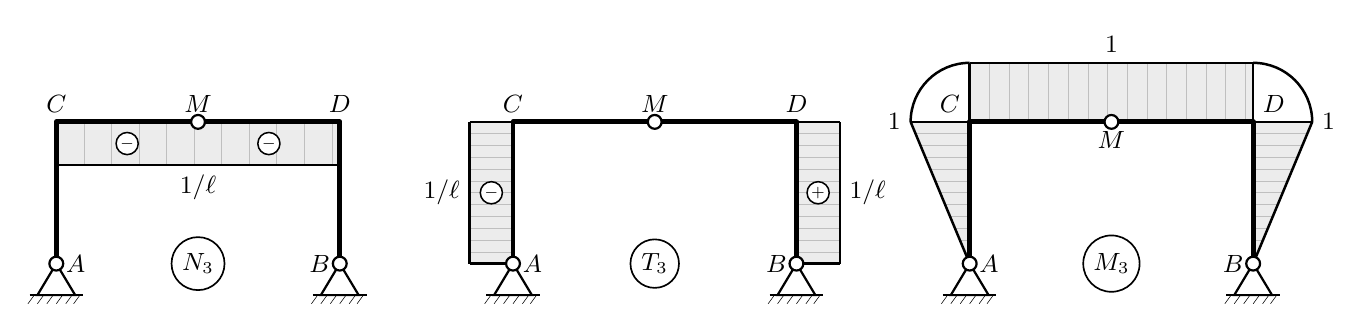
\begin{tikzpicture}[
					trave/.style={line width=1.8pt, line cap=round, line join=round, black},
					terra/.style={line width=0.8pt, black},
					diag/.style={line width=0.90pt, black},
					nodoV/.style={circle, fill=white, draw=black,
						inner sep=0pt, minimum size=5.0pt, line width=0.80pt},
					segno/.style={circle, draw=black, fill=white, inner sep=0pt,
						minimum size=8pt, font=\tiny, line width=0.55pt},
					etlab/.style={circle, draw=black, line width=0.6pt,
						fill=white, inner sep=2pt, font=\small},
					lab/.style={font=\small},
					]
					
					\def\L{1.80}
					\def\SEP{5.80}
					\def\dNt{0.55}   % N₃ traverso: 1/ℓ → 0.55 cm
					\def\dTt{0.55}   % T₃ montanti: 1/ℓ → 0.55 cm
					\def\dMt{0.75}   % M₃: M=1 → 0.75 cm
					
					\def\portale{\draw[trave](0,0)--(0,\L)--(2*\L,\L)--(2*\L,0);}
					\def\cernieraA{%
						\draw[terra](0,0)--(-0.24,-0.40)--(0.24,-0.40)--cycle;
						\draw[terra](-0.34,-0.40)--(0.34,-0.40);
						\foreach \x in {-0.28,-0.16,-0.04,0.08,0.20,0.30}
						\draw[very thin](\x,-0.40)--++(-0.08,-0.11);
						\node[nodoV]at(0,0){};}
					\def\cernieraB{%
						\draw[terra](2*\L,0)--(2*\L-0.24,-0.40)--(2*\L+0.24,-0.40)--cycle;
						\draw[terra]({2*\L-0.34},-0.40)--({2*\L+0.34},-0.40);
						\foreach \x in {-0.28,-0.16,-0.04,0.08,0.20,0.30}
						\draw[very thin]({2*\L+\x},-0.40)--++(-0.08,-0.11);
						\node[nodoV]at(2*\L,0){};}
					
					%%═══ PANNELLO (a) — N₃ ═════════════════════════════════════════════════
					%% N = 0 sui montanti, compressione 1/ℓ uniforme sul traverso (sotto)
					\begin{scope}[xshift=0cm]
						\fill[gray!15](0,{\L-\dNt})--(2*\L,{\L-\dNt})--(2*\L,\L)--(0,\L)--cycle;
						\foreach \x in {0.35,0.70,...,3.50}
						{\draw[gray!50,very thin](\x,{\L-\dNt})--(\x,\L);}
						\draw[diag](0,{\L-\dNt})--(2*\L,{\L-\dNt});
						\portale \cernieraA \cernieraB
						\node[nodoV]at(\L,\L){};
						\node[segno]at({0.5*\L},{\L-\dNt/2}){$-$};
						\node[segno]at({1.5*\L},{\L-\dNt/2}){$-$};
						\node[below=0.04,lab]at(\L,{\L-\dNt}){$1/\ell$};
						\node[right,lab]at(0,0){$A$};
						\node[left,lab]at(2*\L,0){$B$};
						\node[above,lab]at(0,\L){$C$};
						\node[above,lab]at(2*\L,\L){$D$};
						\node[above,lab]at(\L,\L){$M$};
						\node[etlab]at(\L,{0}){$N_3$};
					\end{scope}
					
					%%═══ PANNELLO (b) — T₃ ═════════════════════════════════════════════════
					%% T negativo su AC (esterno=sinistra), positivo su BD (esterno=destra), nullo sul traverso
					\begin{scope}[xshift=\SEP cm]
						%% T montante sinistro (negativo, esterno = sinistra)
						\fill[gray!15]({-\dTt},0)--(0,0)--(0,\L)--({-\dTt},\L)--cycle;
						\foreach \y in {0.15,0.30,...,1.75}
						{\draw[gray!50,very thin]({-\dTt},\y)--(0,\y);}
						\draw[diag]({-\dTt},0)--({-\dTt},\L);
						\draw[diag]({-\dTt},0)--(0,0);
						\draw[diag]({-\dTt},\L)--(0,\L);
						%% T montante destro (positivo, esterno = destra)
						\fill[gray!15](2*\L,0)--({2*\L+\dTt},0)--({2*\L+\dTt},\L)--(2*\L,\L)--cycle;
						\foreach \y in {0.15,0.30,...,1.75}
						{\draw[gray!50,very thin](2*\L,\y)--({2*\L+\dTt},\y);}
						\draw[diag]({2*\L+\dTt},0)--({2*\L+\dTt},\L);
						\draw[diag](2*\L,0)--({2*\L+\dTt},0);
						\draw[diag](2*\L,\L)--({2*\L+\dTt},\L);
						\portale \cernieraA \cernieraB
						\node[nodoV]at(\L,\L){};
						\node[segno]at({-\dTt/2},{\L*0.50}){$-$};
						\node[segno]at({2*\L+\dTt/2},{\L*0.50}){$+$};
						\node[left=0.04,lab]at({-\dTt},{\L*0.50}){$1/\ell$};
						\node[right=0.04,lab]at({2*\L+\dTt},{\L*0.50}){$1/\ell$};
						\node[right,lab]at(0,0){$A$};
						\node[left,lab]at(2*\L,0){$B$};
						\node[above,lab]at(0,\L){$C$};
						\node[above,lab]at(2*\L,\L){$D$};
						\node[above,lab]at(\L,\L){$M$};
						\node[etlab]at(\L,{0}){$T_3$};
					\end{scope}
					
					%%═══ PANNELLO (c) — M₃ ═════════════════════════════════════════════════
					%% M lineare sui montanti (0 in A/B, 1 in C/D, entrambi verso l'esterno)
					%% M uniforme sul traverso (valore 1, sopra = lato teso)
					\begin{scope}[xshift={2*\SEP cm}]
						%% M montante sinistro (triangolo a sinistra: 0 in A, 1 in C)
						\fill[gray!15](0,0)--(-\dMt,\L)--(0,\L)--cycle;
						\begin{scope}
							\clip(0,0)--(-\dMt,\L)--(0,\L)--cycle;
							\foreach \y in {0.15,0.30,...,1.75}
							{\draw[gray!50,very thin]({-\dMt-0.1},\y)--(0.1,\y);}
						\end{scope}
						\draw[diag](0,0)--(-\dMt,\L);
						\draw[diag](-\dMt,\L)--(0,\L);
						%% M montante destro (triangolo a destra: 0 in B, 1 in D)
						\fill[gray!15](2*\L,0)--({2*\L+\dMt},\L)--(2*\L,\L)--cycle;
						\begin{scope}
							\clip(2*\L,0)--({2*\L+\dMt},\L)--(2*\L,\L)--cycle;
							\foreach \y in {0.15,0.30,...,1.75}
							{\draw[gray!50,very thin](2*\L-0.1,\y)--({2*\L+\dMt+0.1},\y);}
						\end{scope}
						\draw[diag](2*\L,0)--({2*\L+\dMt},\L);
						\draw[diag]({2*\L+\dMt},\L)--(2*\L,\L);
						%% M traverso (uniforme, sopra: rettangolo di altezza dMt)
						\fill[gray!15](0,\L)--(2*\L,\L)--(2*\L,{\L+\dMt})--(0,{\L+\dMt})--cycle;
						\begin{scope}
							\clip(0,\L)--(2*\L,\L)--(2*\L,{\L+\dMt})--(0,{\L+\dMt})--cycle;
							\foreach \x in {0.25,0.50,...,3.55}
							{\draw[gray!50,very thin](\x,\L)--(\x,{\L+\dMt});}
						\end{scope}
						\draw[diag](0,{\L+\dMt})--(2*\L,{\L+\dMt});   % linea superiore
						\draw[diag](0,\L)--(0,{\L+\dMt});              % chiusura sinistra (visibile)
						\draw[diag](2*\L,\L)--(2*\L,{\L+\dMt});        % chiusura destra (visibile)
						%% Archetti di continuità in C e D (stessa geometria di M₀)
						\draw[diag](-\dMt,\L) arc(180:90:\dMt);          % C: col.sin → trav
						\draw[diag](2*\L,{\L+\dMt}) arc(90:0:\dMt);      % D: trav → col.des
						%% Struttura
						\portale \cernieraA \cernieraB
						\node[nodoV]at(\L,\L){};
						%% Valori
						\node[left=0.04,lab]at(-\dMt,\L){$1$};
						\node[right=0.04,lab]at({2*\L+\dMt},\L){$1$};
						\node[above=0.04,lab]at(\L,{\L+\dMt}){$1$};
						%% Nodi
						\node[right,lab]at(0,0){$A$};
						\node[left,lab]at(2*\L,0){$B$};
						\node[above left,lab]at(0,\L){$C$};
						\node[above right,lab]at(2*\L,\L){$D$};
						\node[below=0.04,lab]at(\L,\L){$M$};
						\node[etlab]at(\L,{0}){$M_3$};
					\end{scope}
					
				\end{tikzpicture}
			}%
			\caption{Autosoluzione~$3$ ($\chi_3 = 1$, coppia unitaria in~$M$):
				diagrammi di $N_3$, $T_3$ e $M_3$ sul portale a tre cerniere.
				Gli archetti in~$C$ e ~$D$ indicano la continuità del momento flettente
				ai due nodi rigidi.}
			\label{fig:portale_autosoluzione3}
		\end{figure}
